\section{Towards a KM Framework}

%Constraints for such a framework, add two examples as boxes.


\begin{figure}
    \centering
    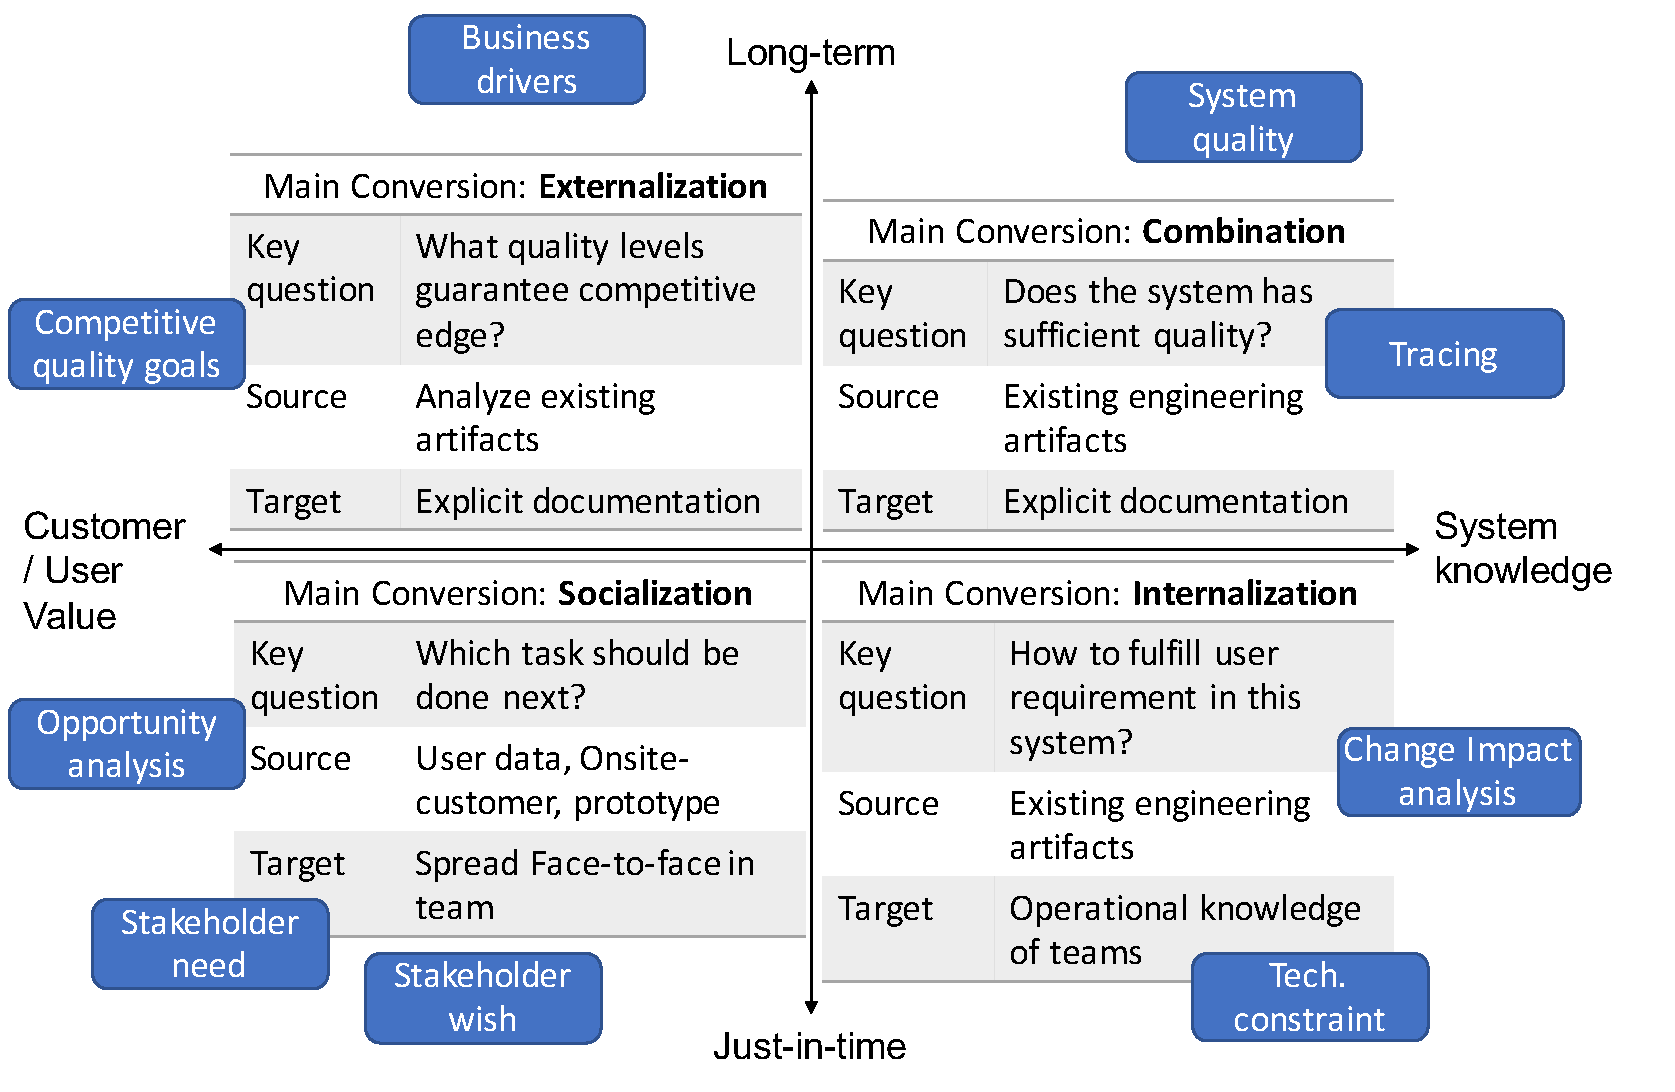
\includegraphics[width=\columnwidth]{figs/km-framework}
    \caption{Towards a Knowledge Management Framework for Agile Quality Requirements Management: Aligning knowledge conversion with our propositions.}
    \label{fig:km_conversion}
\end{figure}




Safety and security are examples of two quality requirements that cannot be managed purely JIT. 
We believe that future research will show similar considerations to apply to all quality requirements, since they are typically related to architecture,  %, whereas functional requirements influence data structures, algorithms, and design patterns. 
%As we have pointed out above, quality requirements
and tend to build on knowledge as much as on software structures, although both need to come together.

In the above-mentioned SecVolution case, an ontology plays a central role of managing knowledge. %The input to that ontology comes from earlier experiences (of attacks), external published warnings (of vulnerabilities), and from insights of security experts. 
Earlier experiences (of attacks), external published warnings (of vulnerabilities), and  insights of security experts are encoded in the ontology, which can then be applied  %, the security frames etc,
%it can be applied 
to natural-language  requirements (Fig. \ref{fig:nnnOben}). 


There are obvious technical challenges involved in building such a knowledge infrastructure. It turned out to be at least equally challenging to solicit, interpret, and engineer the knowledge. Initially, most of that knowledge resides in people and needs to be externalized \cite{Nonaka1995} before it can be encoded and stored in an ontology. Therefore, extracting implicit or even tacit knowledge from people is %one of the focus areas within SecVolution. This step is 
essential and not just a side-issue. 
%Similar to the experience reported in , t
Tapping human knowledge and experience is almost a discipline by itself \cite{Schneider2009}. 
Making a knowledge management infrastructure effective requires taking the social and socio-technical challenges seriously. 
%The central part in Fig. \ref{fig:nnnOben} is the technological infrastructure for managing explicit knowledge. 
Based on these observations, Schneider presents an experience life cycle \cite{Schneider2009} in software engineering (Fig. \ref{fig:nnnUnten}): Activation and collection are  devoted to techniques and tools for attracting implicit or tacit knowledge into the system. 
% For example, the by-product approach has been used for soliciting experience as a by-product of other tasks that need to be conducted anyway \cite{Schneider2006}. 
A purely technocratic view \cite{Earl2001} tends to neglect the left-hand input block. Along the same lines, many experiences (or knowledge items collected) are never actively disseminated. Thus, they remain useless.
%
%
%\ugh{Fig: der Kreis mit dne vier Aktivitäten rund um den Computer: siehe figs.pptx.    }
%
\begin{figure}[t]
        \centering
    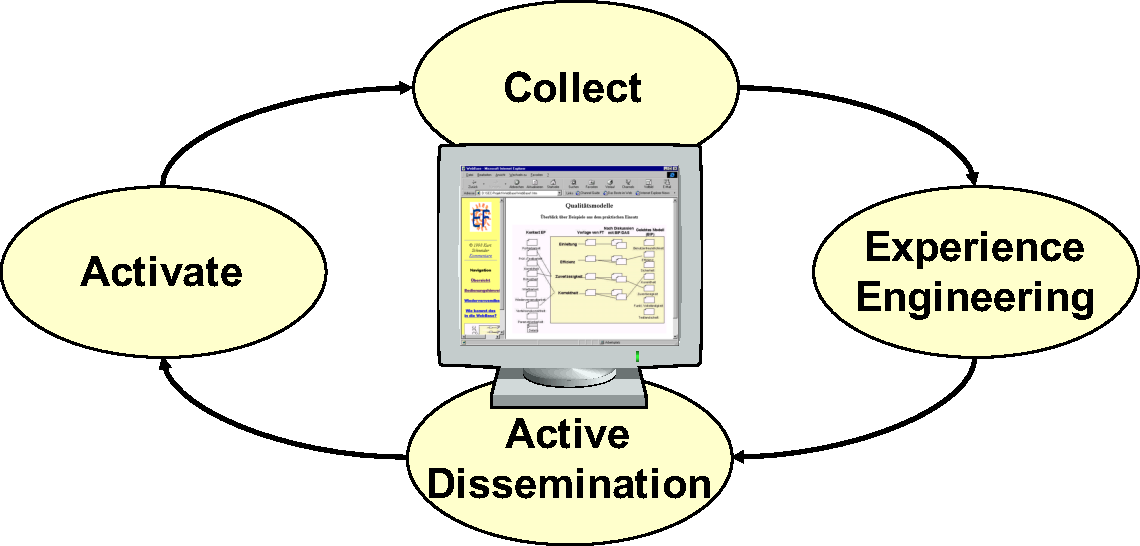
\includegraphics[width=0.7\columnwidth]{figs/nnnUnten}
    \caption{Life-cycle of experiences, iterating around exp. base.}
    \label{fig:nnnUnten}
\end{figure}
%
%
Experts need to be made aware of the valuable knowledge they have (\emph{activate}); there must be support to collect that information once it surfaces (\emph{collect}, e.g. as a by-product of other tasks that need to be conducted anyway \cite{Schneider2006}). 
Usually, the knowledge cannot be collected in exactly the same form that is most appropriate for reuse. Following Basili’s \cite{Basili1994} terminology, we call the activity of merging, comparing, and reformatting ``\emph{experience and knowledge engineering}''. Finally, the resulting knowledge must be delivered to where it is needed, when it is needed, and in the most adequate form. In the SecVolution example, knowledge ends up in an ontology and is automatically applied to natural-language requirements. This is a very clear and technically sophisticated way of distribution. In other cases, knowledge will need to be presented to developers, requiring them to understand and apply it. % (e.g., for performance requirements).

Figures \ref{fig:km_conversion} and \ref{fig:nnnUnten} sketch the core of a knowledge management infrastructure for quality requirements: Fig \ref{fig:nnnUnten}  stresses the iterative nature of experience or knowledge about a quality aspect. 
Such an iterative process is applicable to JIT as well as to long-term requirements. Fig. \ref{fig:km_conversion} highlights different types of sources and the main knowledge operations conducted. %JIT requirements for mitigating a new vulnerability if (and only if) security was continuously maintained. 
JIT and long-term requirements are not a contradiction, but need to complement each other.
We encourage future work to investigate implications for other qualities and on RE processes that support JIT RE based on long-term knowledge.
